\section*{\fontsize{16}{14}\selectfont Aim: Study and usage of OpenProj.}
    
{\bf OpenProj} : OpenProj is an open source, free project management software application or solution. OpenProj operates on multiple platforms including Windows, Mac, 
Linux and Unix. OpenProj is ideal for desktop project management and supports opening Microsoft 
or Primavera files. OpenProj 1.4 is an open source desktop project management 
application. This application is an alternative to Microsoft Project.

OpenProj provides control, tracking and management of projects. To create a new 
project the only field required is the Project Name on the Create New Project 
window and the start date of the project can be change it if you don't want to 
start the day that you're creating your project. You can add tasks in the Gantt 
diagram providing the start and end dates of each task; also you can add 
information to each task such the predecessors and successors tasks, resources, 
notes, etc. One great feature is that provides the Work Breakdown Structure
 (WBS) to order and control the tasks of the project for people who manages 
projects this is a very important tool. Another great feature is the Resource

Breakdown Structure (RBS) to define the structure of the resources, teams, 
providers, etc. Task Usage and Resource Usage are features to control your project and provide a good track on it. The Report tool provides information about the current status of your project.

The features of OpenProj are as follows:-
\begin{description}
\item{\textbf{Gantt chart}}:- A Gantt chart is a type of bar chart, developed by Henry Gantt in the 1910s, that illustrates a project schedule. Gantt charts illustrate the start and finish dates of the terminal elements and summary elements of a project. Terminal elements and summary elements comprise the work breakdown structure of the project. Modern Gantt charts also show the dependency (i.e. precedence network) relationships between activities.

\item{\textbf{PERT graph}}:- The Program (or Project) Evaluation and Review Technique, commonly abbreviated PERT, is a statistical tool, used in project management, that is designed to analyze and represent the tasks involved in completing a given project. First developed by the United States Navy in the 1950s, it is commonly used in conjunction with the critical path method (CPM).

\item {\textbf{Resource Breakdown Structure (RBS) chart}}:- In project management, the resource breakdown structure (RBS) is a hierarchical list of resources related by function and resource type that is used to facilitate planning and controlling of project work. In some cases, a geographic division may be preferred. Each descending (lower) level represents an increasingly detailed description of the resource until small enough to be used in conjunction with the work breakdown structure (WBS) to allow the work to be planned, monitored and controlled.

\item{\textbf{Work Breakdown Structure (WBS) char}t}: - A work breakdown structure (WBS), in project management and systems engineering, is a deliverable oriented decomposition of a project into smaller components.A work breakdown structure element may be a product, data, service, or any combination thereof.

\end{description}


Steps of installation of OpenProj:
\begin{figure}[!th]
\centering

\includegraphics[width=0.7\linewidth]{input/images/image30.jpeg}
\caption{Download by clicking here}
\label{fig:image1}
\end{figure}

\begin{figure}[!th]
\centering
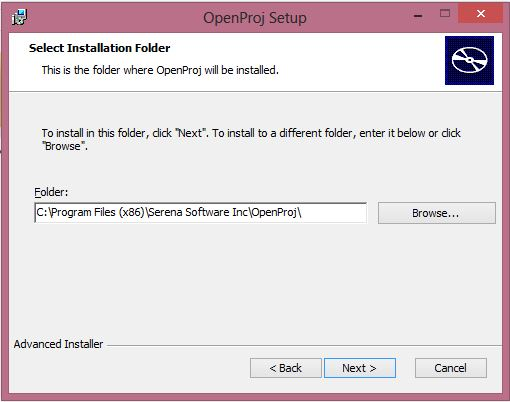
\includegraphics[width=0.7\linewidth]{input/images/image32.jpeg}
\label{fig:image1}
\caption{Click Next}
\end{figure}

\begin{figure}[!th]
\centering
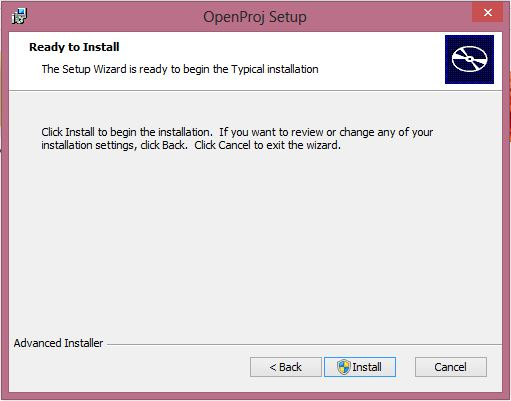
\includegraphics[width=0.7\linewidth]{input/images/image33.jpeg}
\label{fig:image1}
\caption{Click Install}
\end{figure}

\begin{figure}[!th]
\centering
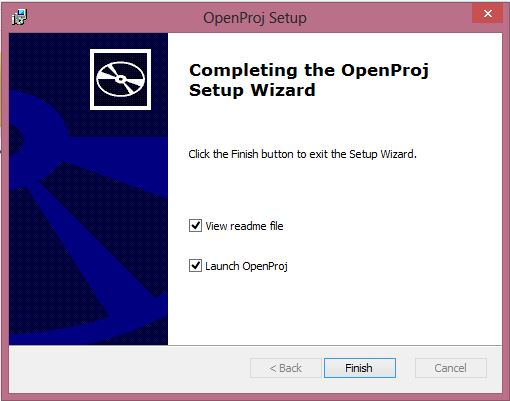
\includegraphics[width=0.7\linewidth]{input/images/image34.jpeg}
\label{fig:image1}
\caption{Click Finish}
\end{figure}

\begin{figure}[!ht]
\centering
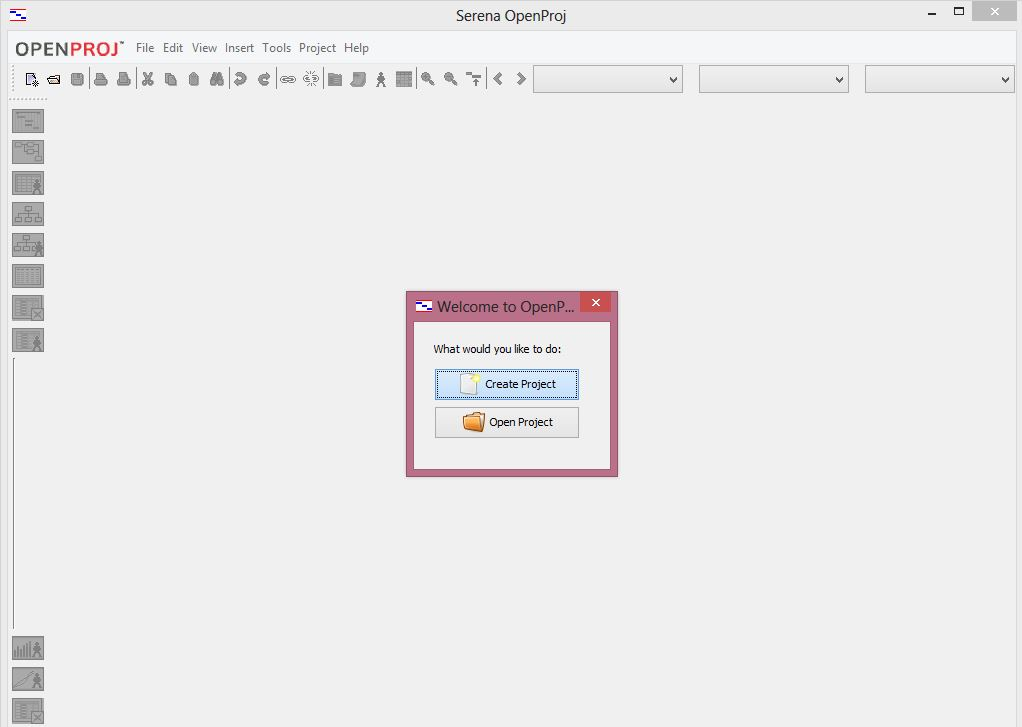
\includegraphics[width=0.7\linewidth]{input/images/image35.jpeg}
\label{fig:image1}
\caption{ Create Project Name: Web-Octave}
\end{figure}

\begin{figure}[!ht]
\centering
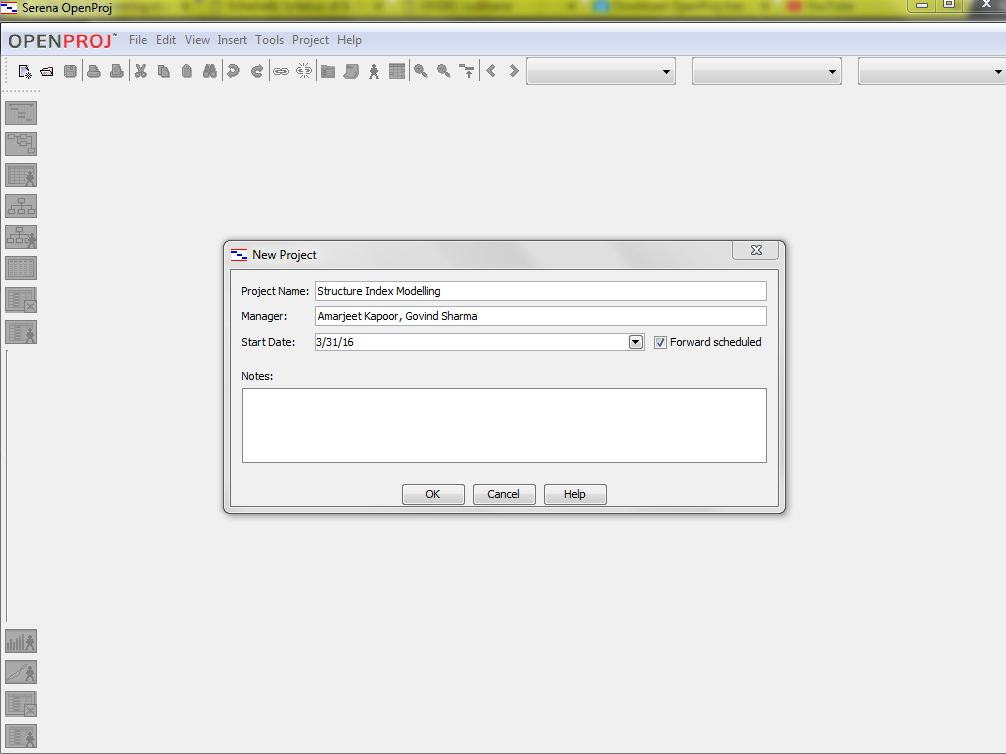
\includegraphics[width=0.7\linewidth]{input/images/image36.jpeg}
\label{fig:image1}
\caption{ Click OK}
\end{figure}



